% Apresentações em widescreen. Outros valores possíveis: 1610, 149, 54, 43 e 32.
% Por padrão, as apresentações são no formato 4:3 (sem o aspectratio).
\documentclass[aspectratio=169]{beamer}	 	

\usetheme[progressbar=frametitle]{metropolis}
\usepackage{appendixnumberbeamer}

\usepackage{booktabs}
\usepackage[scale=2]{ccicons}

\usepackage{pgfplots}
\usepgfplotslibrary{dateplot}

\usepackage{xspace}
\newcommand{\themename}{\textbf{\textsc{metropolis}}\xspace}


% ---
% PACOTES
% --
\usepackage[alf]{abntex2cite}		% Citações padrão ABNT
\usepackage[brazil]{babel}		    % Idioma do documento
\usepackage{color}			       % Controle das cores
\usepackage[T1]{fontenc}		  % Selecao de codigos de fonte.
\usepackage{graphicx}			    % Inclusão de gráficos
\usepackage[utf8]{inputenc}		   % Codificacao do documento (conversão automática dos acentos)
\usepackage{multirow}
\usepackage{threeparttable}
\usepackage[capposition=top]{floatrow}
\usepackage{txfonts}			 % Fontes virtuais
\usepackage{ragged2e}
\usepackage{etoolbox}
\usepackage{lipsum}
\usepackage{amssymb}
% ---

% ---
% Minhas Definições
% ---

%Deixando o Caption alinhado a esquerda mesmo com quebra de linha
\usepackage[labelfont=bf, justification=justified,singlelinecheck=true]{caption}

%Justificando o corpo do texto
\renewcommand{\raggedright}{\leftskip=0pt \rightskip=0pt plus 0cm} 

% Colocando numero de paginas no slide
\setbeamertemplate{footline}[frame number]{}
\setbeamertemplate{caption}[numbered]{}

% Tela cheia
%\hypersetup{pdfpagemode=FullScreen}
% ---


% --- Informações do documento ---
%\logo{
\includegraphics[scale=0.15]{figuras/logo.png}}
\title{Um Ambiente Virtual de Aprendizagem para Auxiliar no Processo de Ensino e Aprendizagem de Matemática}
\author[]{Marciano Machado Saraiva}
\institute{
Orientador: Prof. Me. Samy Soares Passos de Sá\\[2 ex]
Universidade Federal do Ceará
	    \par
	    Bacharel em Sistemas de Informação}
\date{\today}
% ---

% ----------------- INÍCIO DO DOCUMENTO --------------------------------------
\begin{document}

% ----------------- NOVO SLIDE --------------------------------
\begin{frame}

    \titlepage

\end{frame}

% ----------------- NOVO SLIDE --------------------------------
\begin{frame}{Roteiro}
	\tableofcontents
\end{frame}

%% ----------------- NOVO SLIDE --------------------------------
\section{Introdução}

\begin{frame}{Introdução: Motivação}

\begin{figure}[H]
	\centering
	\caption{Desepemho do Brasil no PISA}
	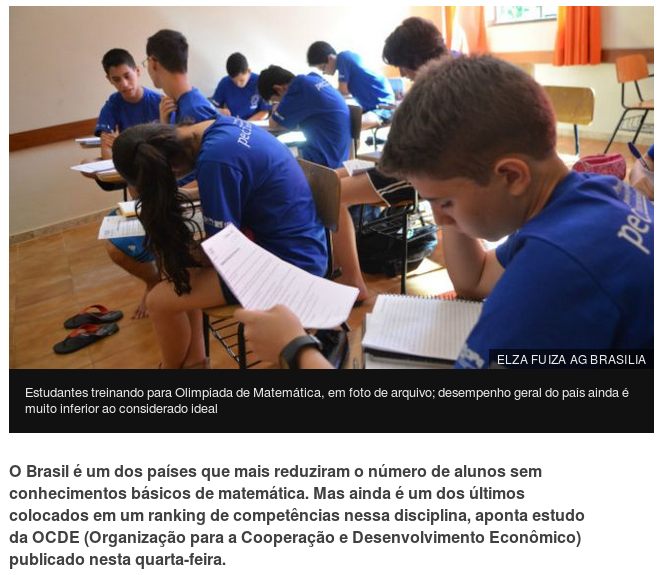
\includegraphics[width=7cm]{figuras/motivacao.png}
	\floatfoot{Fonte: \cite{pisabbc2016}}
	\end{figure}

\end{frame}

% ----------------- NOVO SLIDE --------------------------------
\begin{frame}
\frametitle{Introdução: Objetivos}

\begin{block}{Objetivo Geral}
	Desenvolver um Ambiente Virtual de Aprendizagem para auxiliar no processo de ensino e aprendizagem de matemática de alunos dentro e fora da sala de aula.
	\pause
\end{block}

\begin{block}{Objetivos Específicos}

\begin{itemize}
  \item Levantar os requisitos do sistema.
  \pause
  \item Desenvolver os módulos com funções de administração do sistema.
  \pause
  \item Desenvolver os módulos com funções que serão utilizadas pelos estudantes aplicando técnicas de Gamificação.
  \pause
  \item Avaliar a qualidade de uso da interface da plaforma desenvolvida através da aplicação de testes de usabilidade e entrevistas com estudantes do ensino médio e universitários.
\end{itemize}

\end{block}

\end{frame}

% ----------------- NOVO SLIDE --------------------------------
\section{Revisão Bibliográfica}

\begin{frame}{Revisão Bibliográfica}
\frametitle{Revisão Bibliográfica: Conceitos Abordados}

\begin{itemize}
	\item Metodologias no Ensino da Matemática
	\item Ambiente Virtual de Aprendizagem
	\item Gamifica\c{c}\~ao
\end{itemize}

\end{frame}

% ----------------- NOVO SLIDE --------------------------------
\begin{frame}{Trabalhos Relacionados}
\frametitle{Revisão Bibliográfica: Trabalhos Relacionados}

\begin{itemize}
	\item KhanAcademy: The one world schoolhouse -- Education reimagined
	\item ActiveMath: A generic and adaptive web-based learning environment
	\item Duolingo: Learn a Language for Free while Helping to Translate the Web
	\item Resolução de problemas em ambientes virtuais de aprendizagem num curso de licenciatura em matemática na modalidade a distância
\end{itemize}

\end{frame}

% ----------------- NOVO SLIDE --------------------------------
\section{Descrição da Proposta}

\setcounter{figure}{0}

\begin{frame}{Descrição da Proposta}

\begin{overprint}
\only<+>{
	\begin{figure}[H]
	\centering
	\caption{Representa\c{c}\~ao do nosso Modelo de Aprendizagem}
	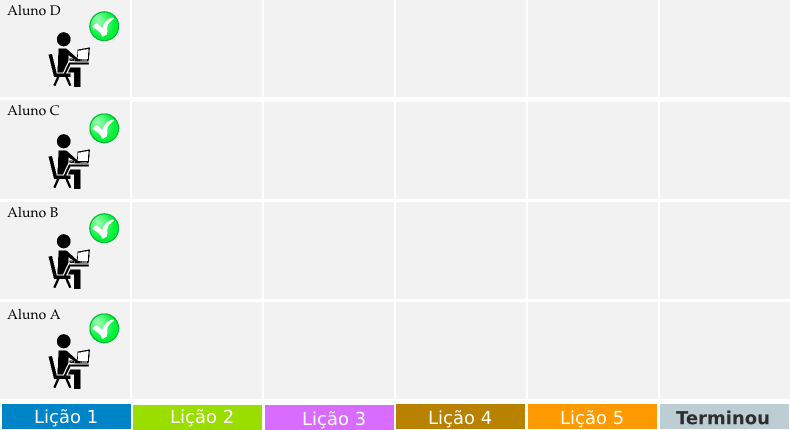
\includegraphics[width=8cm]{figuras/proposta/imagem1.png}
	\floatfoot{Fonte: Elaborada pelo autor}
	\end{figure}
}
\only<+>{
	\begin{figure}[H]
	\centering
	\caption{Representa\c{c}\~ao do nosso Modelo de Aprendizagem}
	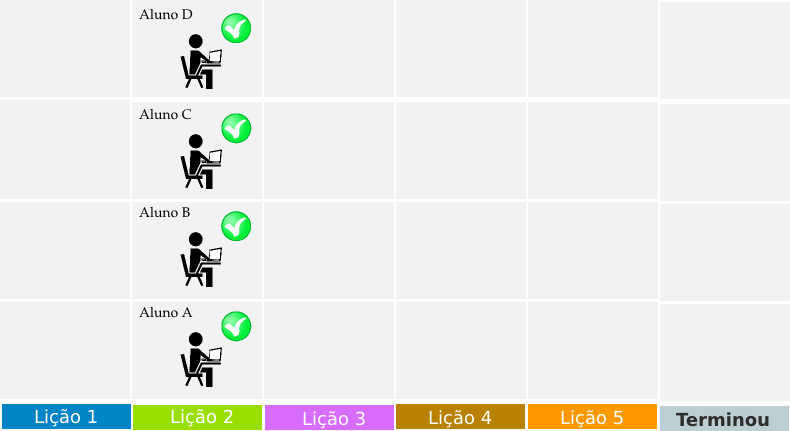
\includegraphics[width=8cm]{figuras/proposta/imagem2.png}
	\floatfoot{Fonte: Elaborada pelo autor}
	\end{figure}
}
\only<+>{
	\begin{figure}[H]
	\centering
	\caption{Representa\c{c}\~ao do nosso Modelo de Aprendizagem}
	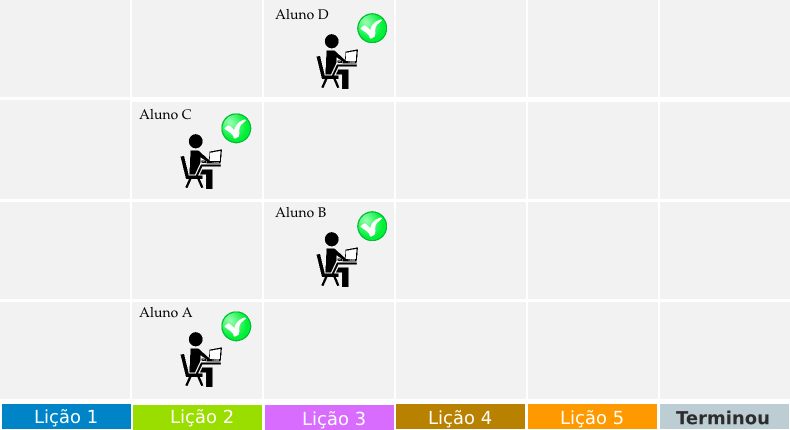
\includegraphics[width=8cm]{figuras/proposta/imagem3.png}
	\floatfoot{Fonte: Elaborada pelo autor}
	\end{figure}
}
\only<+>{
	\begin{figure}[H]
	\centering
	\caption{Representa\c{c}\~ao do nosso Modelo de Aprendizagem}
	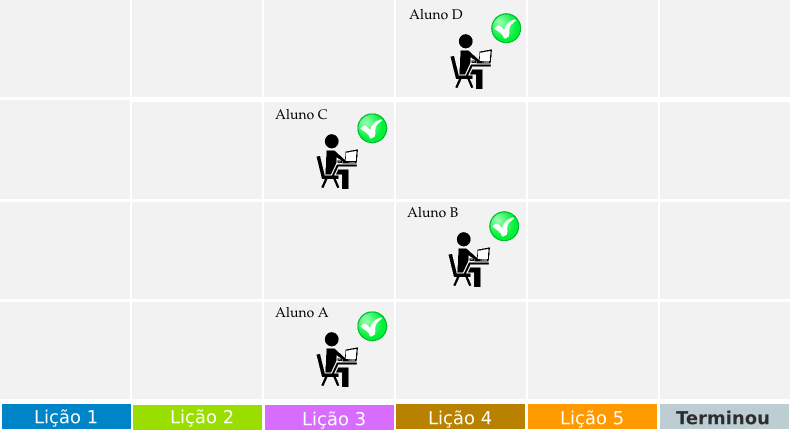
\includegraphics[width=8cm]{figuras/proposta/imagem4.png}
	\floatfoot{Fonte: Elaborada pelo autor}
	\end{figure}
}
\only<+>{
	\begin{figure}[H]
	\centering
	\caption{Representa\c{c}\~ao do nosso Modelo de Aprendizagem}
	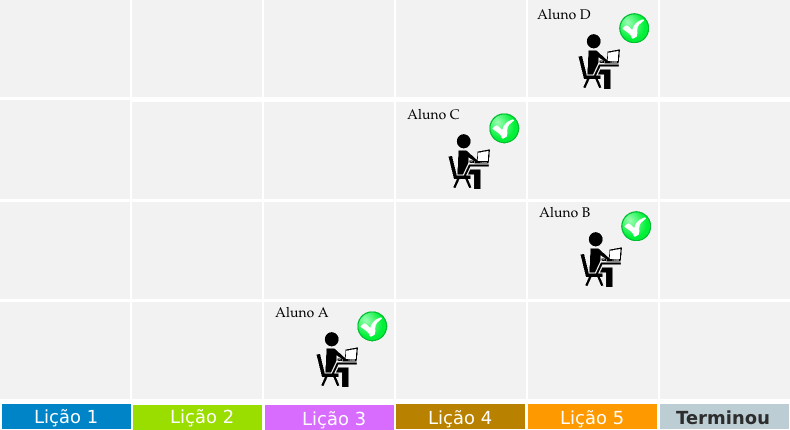
\includegraphics[width=8cm]{figuras/proposta/imagem5.png}
	\floatfoot{Fonte: Elaborada pelo autor}
	\end{figure}
}
\only<+>{
	\begin{figure}[H]
	\centering
	\caption{Representa\c{c}\~ao do nosso Modelo de Aprendizagem}
	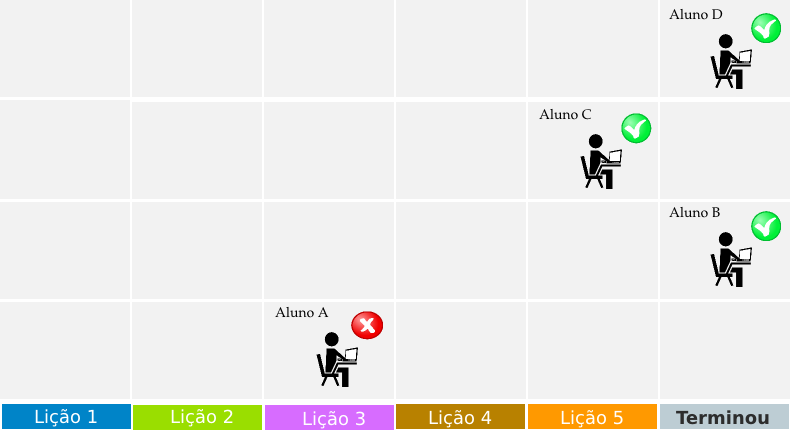
\includegraphics[width=8cm]{figuras/proposta/imagem6.png}
	\floatfoot{Fonte: Elaborada pelo autor}
	\end{figure}
}
\only<+>{
	\begin{figure}[H]
	\centering
	\caption{Representa\c{c}\~ao do nosso Modelo de Aprendizagem}
	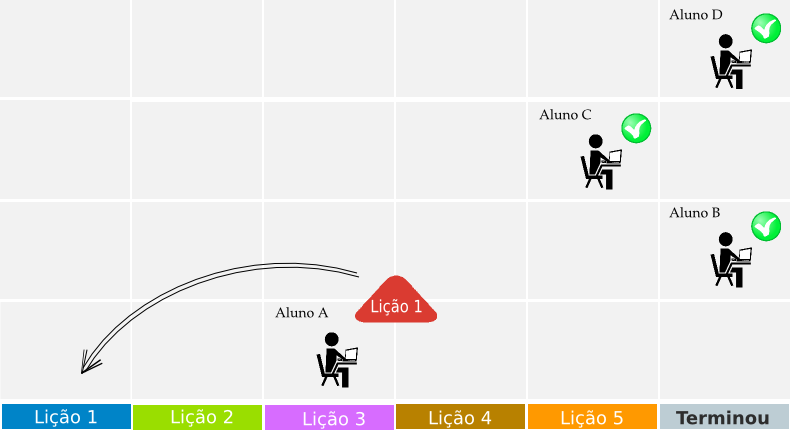
\includegraphics[width=8cm]{figuras/proposta/imagem7.png}
	\floatfoot{Fonte: Elaborada pelo autor}
	\end{figure}
}
\only<+>{
	\begin{figure}[H]
	\centering
	\caption{Representa\c{c}\~ao do nosso Modelo de Aprendizagem}
	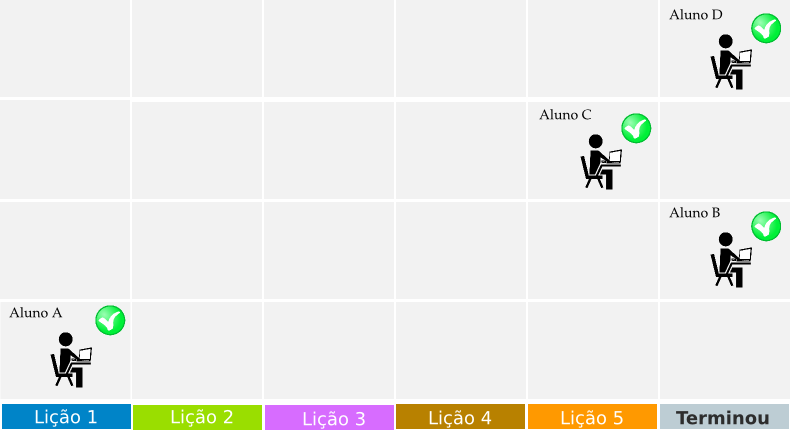
\includegraphics[width=8cm]{figuras/proposta/imagem8.png}
	\floatfoot{Fonte: Elaborada pelo autor}
	\end{figure}
}
\only<+>{
	\begin{figure}[H]
	\centering
	\caption{Representa\c{c}\~ao do nosso Modelo de Aprendizagem}
	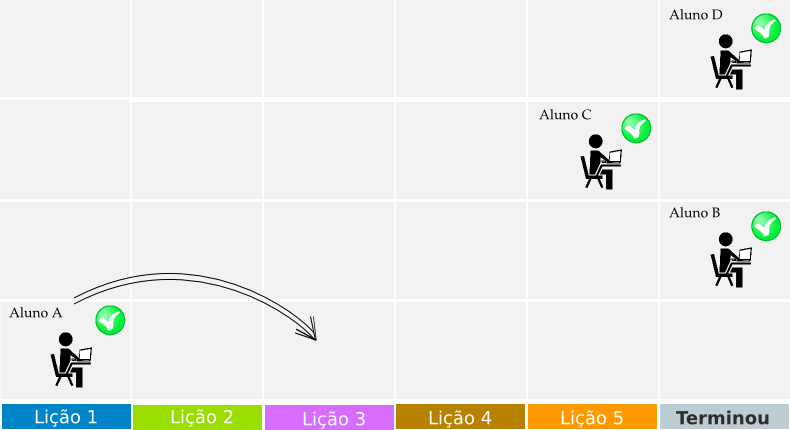
\includegraphics[width=8cm]{figuras/proposta/imagem9.png}
	\floatfoot{Fonte: Elaborada pelo autor}
	\end{figure}
}
\only<+>{
	\begin{figure}[H]
	\centering
	\caption{Representa\c{c}\~ao do nosso Modelo de Aprendizagem}
	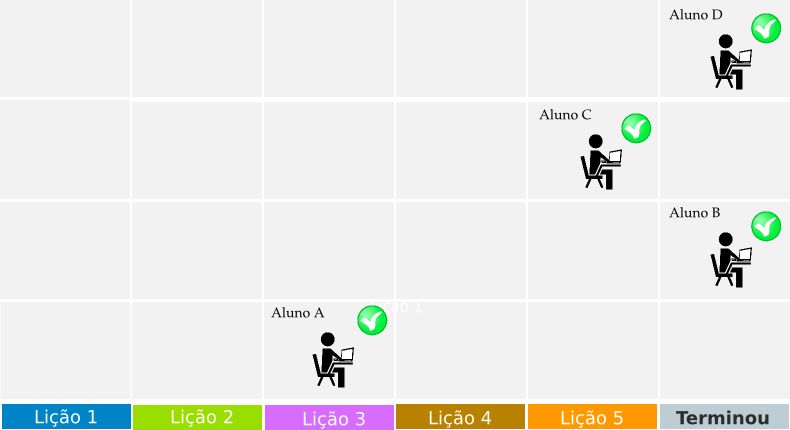
\includegraphics[width=8cm]{figuras/proposta/imagem10.png}
	\floatfoot{Fonte: Elaborada pelo autor}
	\end{figure}
}

\only<+>{
	\begin{figure}[H]
	\centering
	\caption{Representa\c{c}\~ao do nosso Modelo de Aprendizagem}
	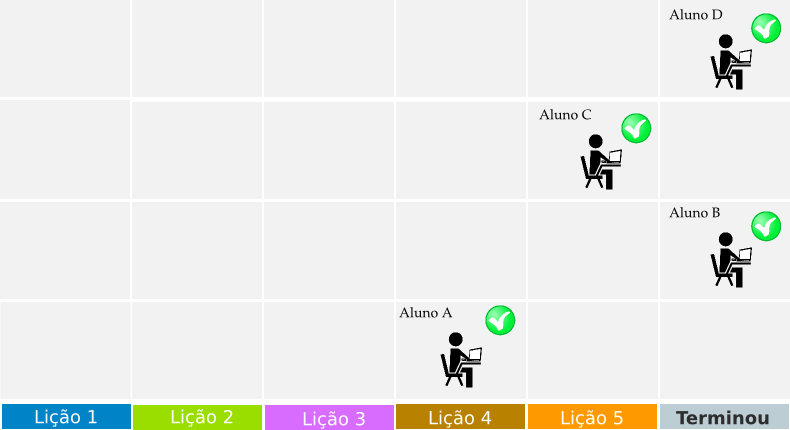
\includegraphics[width=8cm]{figuras/proposta/imagem11.png}
	\floatfoot{Fonte: Elaborada pelo autor}
	\end{figure}
}

\only<+>{
	\setcounter{figure}{1}
	\begin{figure}[H]
	\centering
	\caption{Estrutura do Problema}
	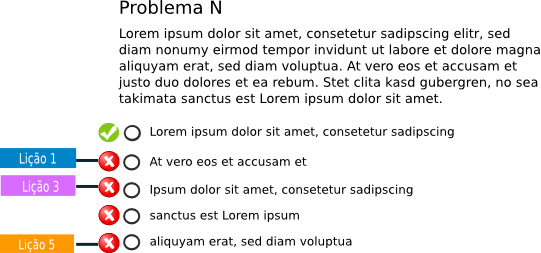
\includegraphics[width=8cm]{figuras/estrutura_problema.png}
	\floatfoot{Fonte: Elaborada pelo autor}
	\end{figure}
}

\end{overprint}

\end{frame}

% ----------------- NOVO SLIDE --------------------------------
\section{Procedimentos Metodológicos}

\begin{frame}{Procedimentos Metodológicos}
	\begin{enumerate}
    	\item Definição do Processo
    	\pause
        \item Levantamento e Análise de Requisitos
		\pause        
        \item Projeto do Sistema
        \pause
        \begin{itemize}
        	\item Arquitetura
        	\pause
        	\item Ferramentas Utilizadas
        	\pause
        \end{itemize}
        \item Implementação do Sistema
        \pause
        \item Verificação e Validação
        \pause
        \item Definição dos Conteúdo para o Sistema
        	\begin{itemize}
        		\item Proposições
        		\item Conjuntos
        	\end{itemize}
    \end{enumerate}
\end{frame}

% ----------------- NOVO SLIDE --------------------------------

\section{Avaliação do Ambiente Virtual de Aprendizagem}

\begin{frame}{Avaliação do Ambiente Virtual de Aprendizagem}
\frametitle{Avaliação do Ambiente Virtual de Aprendizagem}

\begin{itemize}
	\item{Definição do Escopo da Avaliação}
	\pause
	\item{Planejamento}
		\begin{itemize}
			\item Métricas da Avaliação
			\pause
			\item Tarefas
			\pause
			\item Roteiro da Entrevista 
			\pause
		\end{itemize}
	\item Execução
	\pause
	\item Análise dos Resultados
		\begin{itemize}
			\item Tempo de execução das tarefas
			\pause
			\item Número de erros cometidos na execução das tarefas
			\pause
			\item Número de cliques realizados na execução das tarefas
			\pause
			\item Número de perguntas realizadas durante a execução das tarefas
			\pause
			\item Resultados da Entrevista
		\end{itemize}
\end{itemize}

\end{frame}

\begin{frame}{Avaliação do Ambiente Virtual de Aprendizagem}
\frametitle{Avaliação do Ambiente Virtual de Aprendizagem - Extra}

\begin{columns}
\begin{column}{0.8\textwidth}

\begin{table}[H]
\centering
\caption{Uso do ambiente por estudantes de uma turma de Matemática Básica}
\label{tab:uso_ambiente}

\resizebox{\textwidth}{!}{
\begin{tabular}{|l|l|l|l|l|l|}
\hline
\multicolumn{1}{|c|}{\textbf{Estudante}} & \multicolumn{1}{c|}{\textbf{\begin{tabular}[c]{@{}c@{}}Lições Realizadas\\ no AsKMath\end{tabular}}} & \multicolumn{1}{c|}{\textbf{Nota1}} & \multicolumn{1}{c|}{\textbf{Nota2}} & \multicolumn{1}{c|}{\textbf{\begin{tabular}[c]{@{}c@{}}Avanço no \\ AskMath\end{tabular}}} & \multicolumn{1}{c|}{\textbf{\begin{tabular}[c]{@{}c@{}}Avanço nas\\ Notas\end{tabular}}} \\ \hline
E01 & Quase todas de Conjuntos & 2,0 & 8,2 & 3 & 3 \\ \hline
E02 & Todas no tempo certo & 4,8 & 7,5 & 3 & 3 \\ \hline
E03 & Todas de Conjuntos & 2,9 & 7,1 & 3 & 3 \\ \hline
E04 & Todas de Conjuntos & 2,3 & 5,3 & 3 & 3 \\ \hline
E05 & Apenas de Conjuntos & 0,9 & 4,9 & 3 & 3 \\ \hline
E06 & Todas de Conjuntos & 4,0 & 4,8 & 3 & 1 \\ \hline
E07 & Nenhuma & 3,2 & 4,6 & 0 & 2 \\ \hline
E08 & Nenhuma & 1,0 & 4,2 & 0 & 3 \\ \hline
E09 & Nenhuma & 1,5 & 2,9 & 0 & 2 \\ \hline
E10 & Nenhuma & 3,7 & 4,1 & 0 & 1 \\ \hline
E11 & Exercício Moderado & 2,3 & 3,0 & 2 & 1 \\ \hline
E12 & Apenas de Conjuntos & 0,2 & 2,8 & 3 & 3 \\ \hline
\end{tabular}
}
\end{table}

\end{column}
\begin{column}{0.2\textwidth}  %%<--- here

\begin{table}[H]
\centering
\label{my-label}

\resizebox{\textwidth}{!}{
\begin{tabular}{|c|c|c|}
\hline
\multicolumn{3}{|c|}{\textbf{Legenda}} \\ \hline
\textbf{Unidade} & \textbf{\begin{tabular}[c]{@{}c@{}}Avanços no\\ AskMath\end{tabular}} & \textbf{\begin{tabular}[c]{@{}c@{}}Avanços na \\ Nota\end{tabular}} \\ \hline
0 & Nada & Nada \\ \hline
1 & Pouco & Baixo \\ \hline
2 & Moderado & Médio \\ \hline
3 & Total & Alto \\ \hline
\end{tabular}
}

\end{table}

\end{column}
\end{columns}


\end{frame}

% ----------------- NOVO SLIDE --------------------------------
\section{Resultados}
\begin{frame}{Resultados}

\begin{block}{Módulos Desenvolvidos}
	\begin{itemize}
		\item Gerenciador de Usuários
		\item Gerenciador de Turmas
		\item Gerenciador de Assuntos
		\item Gerenciador de Lições
		\item Gerenciador de Problemas
		\item Gerenciador de Pontuação
		\item Gerenciador de Progresso
		\item Gerador de Estatísticas
		\item F\'orum de Discussões
	\end{itemize}
\end{block}

\end{frame}

\begin{frame}{Resultados}
	\begin{figure}[H]
	\centering
	\caption{Tela Inicial do Sistema}
	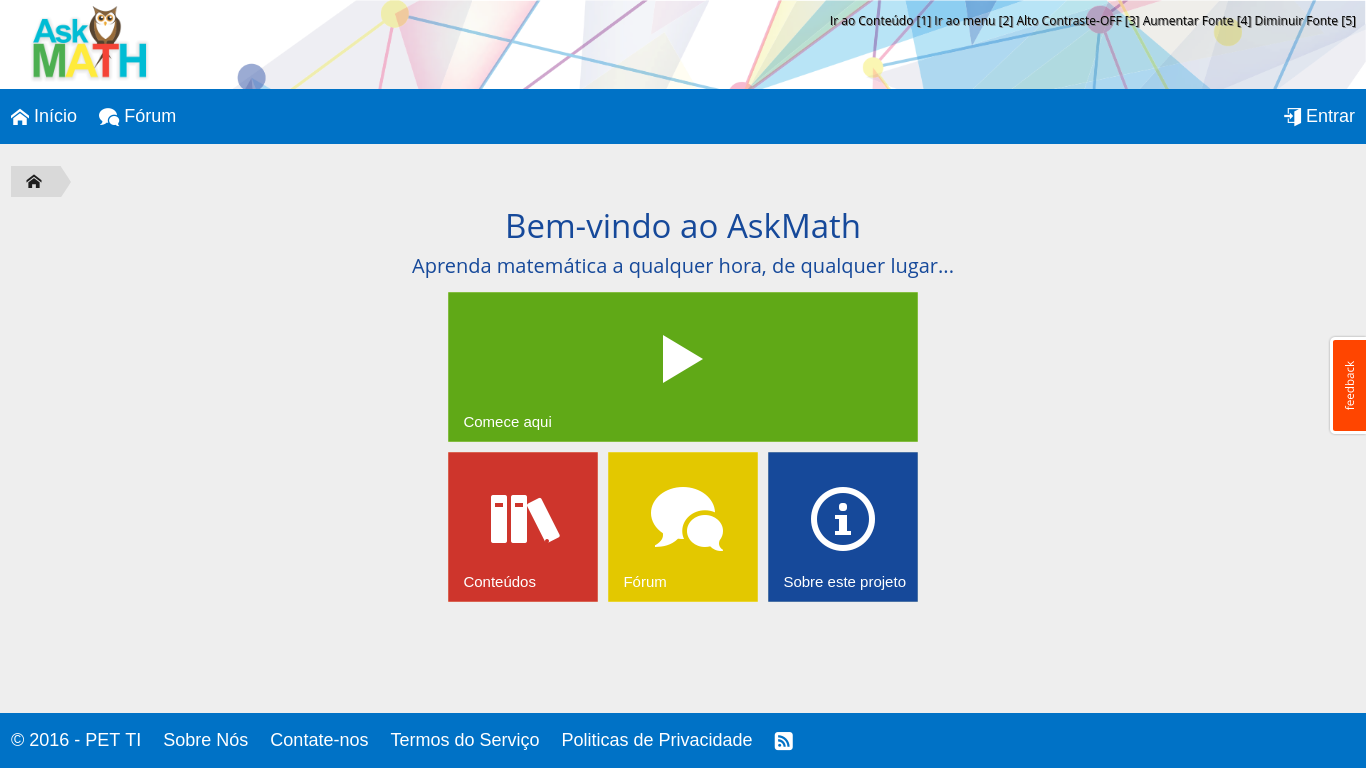
\includegraphics[width=8cm]{figuras/askmath/1.png}
	\floatfoot{Fonte: \url{www.askmath.quixada.ufc.br} }
	\end{figure}
\end{frame}

\begin{frame}{Resultados}
	\begin{figure}[H]
	\centering
	\caption{Tela com lições de Proposições}
	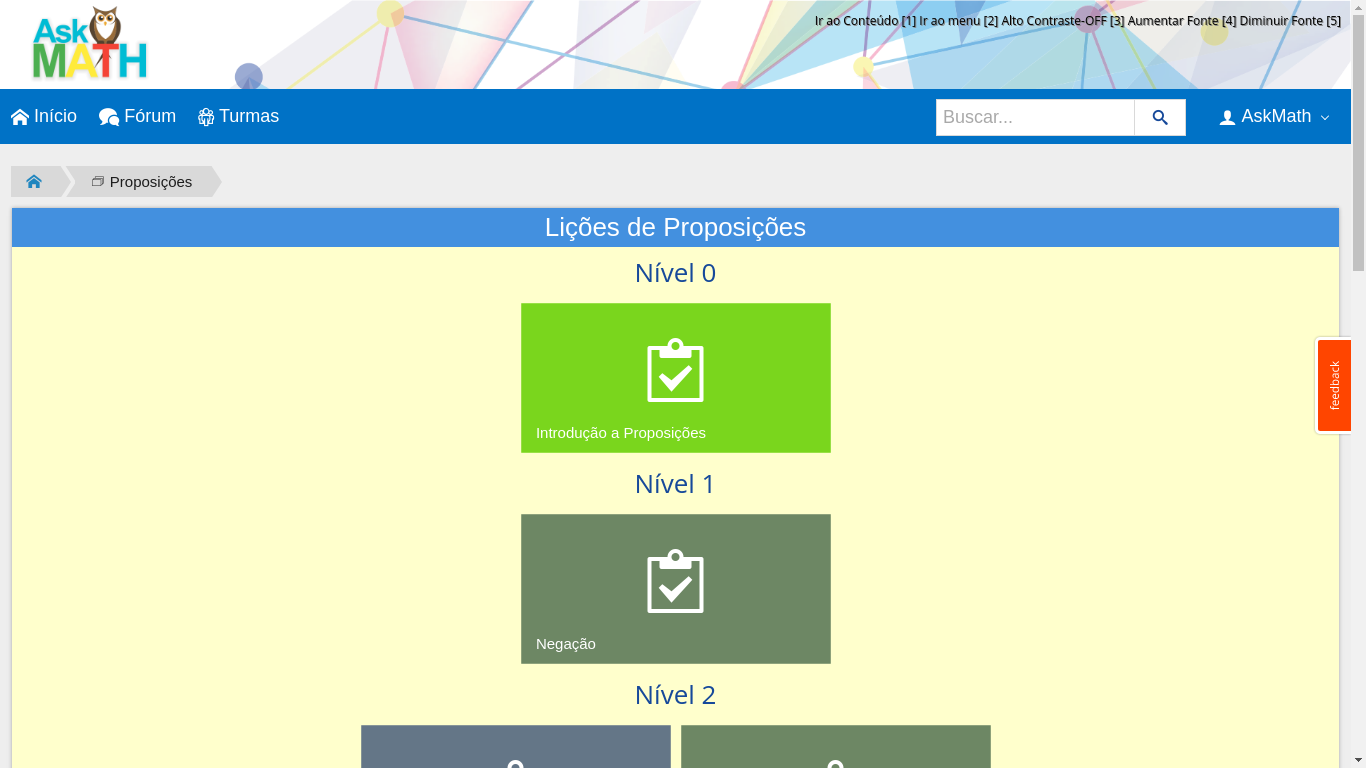
\includegraphics[width=8cm]{figuras/askmath/2.png}
	\floatfoot{Fonte: \url{www.askmath.quixada.ufc.br} }
	\end{figure}
\end{frame}

\begin{frame}{Resultados}
	\begin{figure}[H]
	\centering
	\caption{Tela de problemas do estudante}
	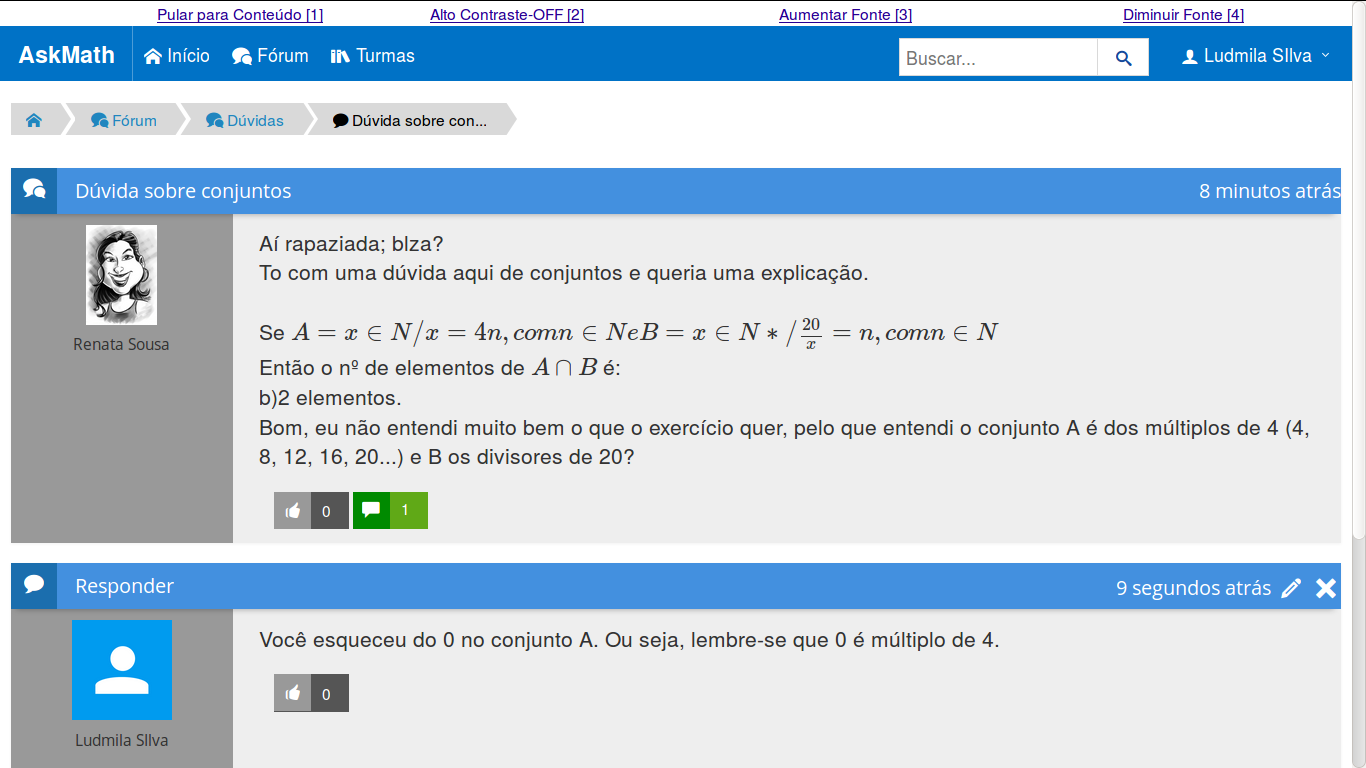
\includegraphics[width=10cm]{figuras/askmath/4.png}
	\floatfoot{Fonte: \url{www.askmath.quixada.ufc.br} }
	\end{figure}
\end{frame}

\begin{frame}{Resultados}
	\begin{figure}[H]
	\centering
	\caption{Tela de uma postagem no fórum}
	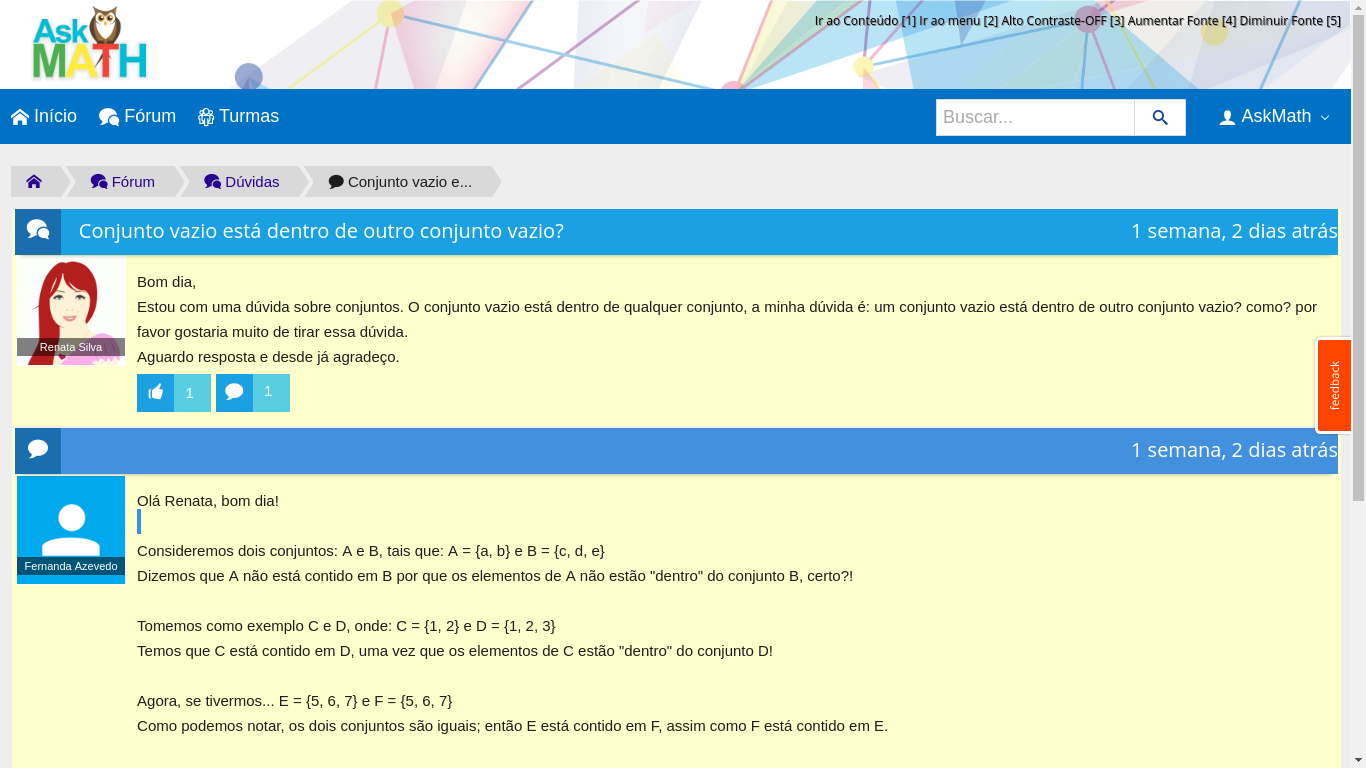
\includegraphics[width=10cm]{figuras/askmath/5.png}
	\floatfoot{Fonte: \url{www.askmath.quixada.ufc.br} }
	\end{figure}
\end{frame}

\begin{frame}{Resultados}
	\begin{figure}[H]
	\centering
	\caption{Tela de administração}
	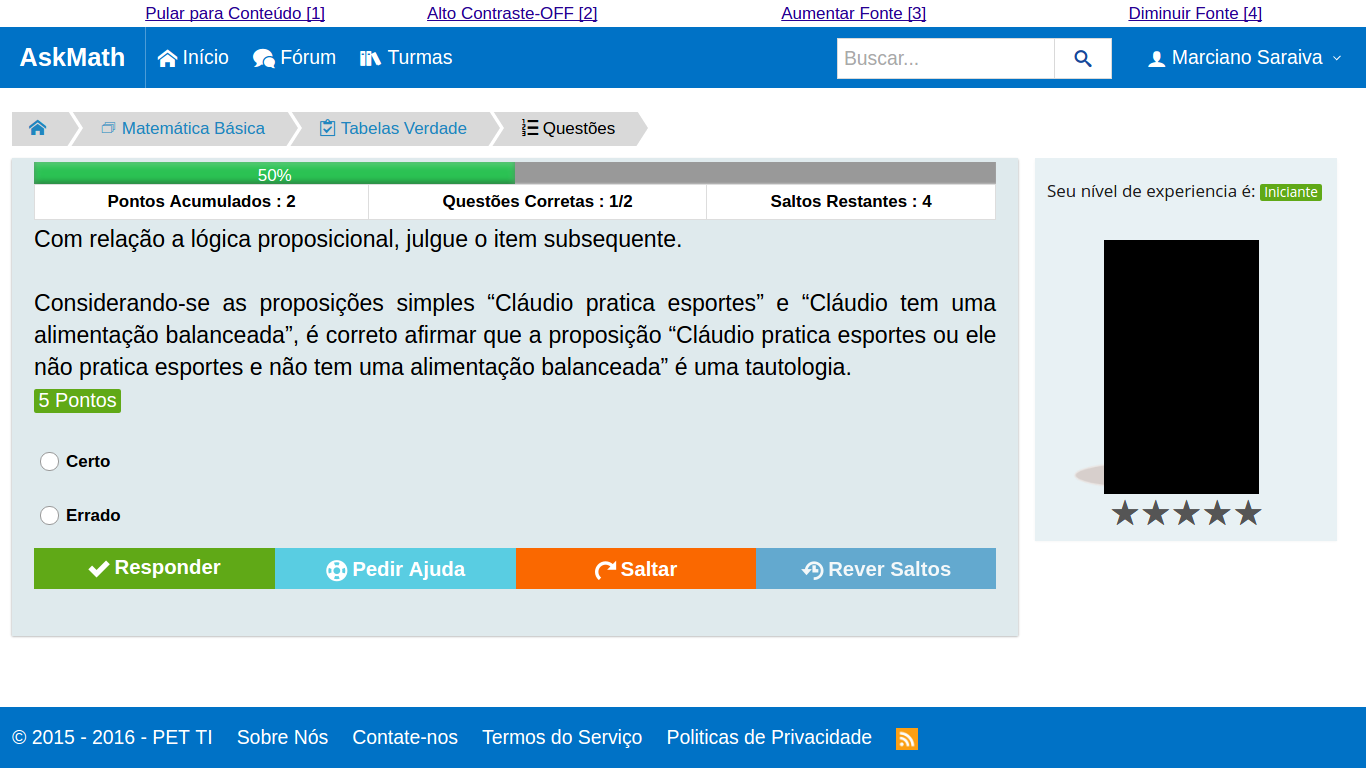
\includegraphics[width=10cm]{figuras/askmath/3.png}
	\floatfoot{Fonte: \url{www.askmath.quixada.ufc.br} }
	\end{figure}
\end{frame}

\begin{frame}{Resultados}
	\begin{figure}[H]
	\centering
	\caption{Tela com problemas do administrador}
	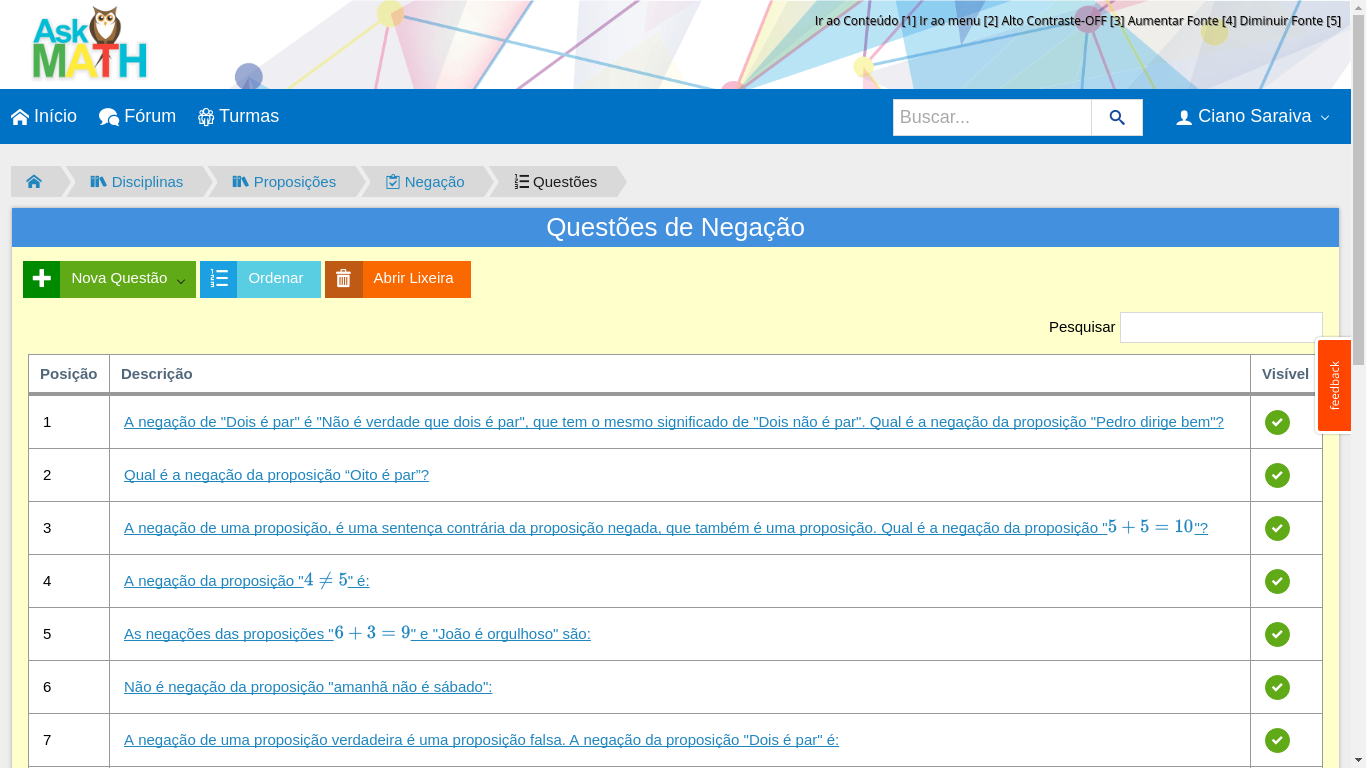
\includegraphics[width=10cm]{figuras/askmath/6.png}
	\floatfoot{Fonte: \url{www.askmath.quixada.ufc.br} }
	\end{figure}
\end{frame}

\section{Conclusão e Trabalhos Futuros}

\begin{frame}{Conclusão}
   \begin{itemize}
   		\item Uso das melhores práticas e padrões em desenvolvimento de \textit{software}.
   		\item Ambiente Propício a prática do conhecimento adquirido na sala de aula.
		\item Complemento ao ensino presencial.
		\item Limitações na solução.
   \end{itemize}
\end{frame}

\begin{frame}{Trabalhos Futuros}
   \begin{itemize}
   		\item Desenvolver um módulo de bate-papo entre os alunos e
professores.
   		\item Adição de conteúdos apresentados através de recursos visuais.
   		\item Melhorias na interface gráfica.
   		\item Avaliar o aprendizado que o sistema pode proporcionar à alunos durante seu uso como complemento ao ensino.
   \end{itemize}
\end{frame}

% ----------------- NOVO SLIDE --------------------------------
\section{Referências}

\begin{frame}[allowframebreaks]{Referências}
	\bibliography{referencias}
\end{frame}

% ----------------- NOVO SLIDE --------------------------------

\begin{frame}
	\begin{columns}
		\begin{column}{3cm}
			
\includegraphics[height=3cm]{figuras/logo.png}
		\end{column}
		\begin{column}{7cm}
			\begin{flushright}
				\centering
				\vskip 0.5cm
				\Huge Obrigado!
			\end{flushright}
		\end{column}
	\end{columns}
\end{frame}


% ----------------- FIM DO DOCUMENTO -----------------------------------------
\end{document}